% =============================================================================
% Appendix: Survey and Survey Build
% =============================================================================
% SPDX-FileCopyrightText: 2026 Drewan Rutherford <RutherfordD@cardiff.ac.uk>
% SPDX-License-Identifier: LPPL-1.3c
% =============================================================================

This appendix covers the unused survey and the incomplete survey build of the game, alongside the supporting material. None of this was distributed due to time constraints. There were three major components to this:

\begin{enumerate}
    \item The landing page, deployed using GitHub Pages,
    \item The special build of the game designed for user evaluation,
    \item A Microsoft forms questionnaire. 
\end{enumerate}

The survey was be be completed synonymously to the player playing through the game, with instructions on both ends on when to switch. This appendix combines all three components into the order that the respondent would interact with them.

The survey build of the game included a basic slide system for containing the test levels. This system allowed for descriptions to appear at the start of slides and hint text. These extra bits of text will not be included here but are visible in the source code (at time of submission), under a slide's \textit{SlideManager} node. Screenshots of the levels are taking in the Godot editor, with the purple background removed.

Each section had a header and a footer slide in Godot which introduced each section or directed the user to answer questions on the survey. These were not all completed, and have been omitted from this appendix. All slide references in the section were taken at time of submission and may have been removed or altered after submission.

\section{Participant Information}

\subsection{Landing Page}

Location \textbf{GitHub Pages}

The landing page was to contain all the required information about the study, including information sheets, and links to the game and survey proper. This was one of the components of the study that was in the draft stages. This were created using markdown making use of GitHub Page's compatibility with markdown.

\begin{fullwidth}
    \begin{quote}
        \textbf{Code Heist User Evaluation}

Hello,

Thanks, for showing interest in participating in my user evaluation for my CM2303 One Semester Individual Project. I am evaluating the use of platformers incorporating programming into their mechanics to teach programming. As part of this I am carrying out a user evaluation of some of the systems created for this.

I am looking for participants aged 18 or over to participate in a user evaluation through playing a few test levels and filling out a survey.

I welcome feedback from people with all levels of experience with both video games and programming (including none at all) to participate.

If you have any questions, please send them to my email listed below.

\textbf{What you will be doing}

To participate, you will being answering some questions whilst playing through a few prototype levels and slides. It will make more sense when you start, and I have detailed instructions below. You will need to use a laptop or PC. Essentially any device with a keyboard and mouse that can display webpages.

Warning: The game doesn’t run equally well on all platforms, for best results use windows and google chrome. Though firefox also works on most platforms, as well as linux. I do not see why MacOS wouldn’t work but its untested.

\textbf{Instructions}

First, you must read the participant information sheet. You can either view it as a pdf or as a webpage.

Once you have done this, open the game and survey simultaneously. This can be in two different tabs, or through opening the survey on your phone either by following the link again, or through the QR code below.

From here, follow the instruction in game and in the survey. You may spend as long as you want on each level in game, however if you want to be done within the 30 minutes, don’t spend more than 4 minutes on each level.

I will not be excepting responses past the [Survey end date]. 

\textbf{Links}

    Participant Information:
        [Links to participant information]

    Game:
        [Link to game]

    Survey:
        [Link to survey]
        
        Or scan the following QR code:
        [QR code leading to the same survey]

\textbf{Contact}

If you have any questions or queries please email me at: [email address].

    \end{quote}
\end{fullwidth}

\subsection{Information (Survey)}

Location: \textbf{Microsoft Forms}

\begin{fullwidth}
    \begin{quote}
        \textbf{Section 1: Information}
    
        In this survey you will be asked some questions about your experience programming, before playing through a few prototype levels whilst answering questions. These questions are designed to evaluate subjective elements of game as part of a user evaluation.
        
        You should have already read the participant information sheet, and have the game open either in a different tab or device.
        
        If you need to go back for either of these things, follow this link: [Link to Landing Page]
    \end{quote}
\end{fullwidth}

\subsection{Information (Godot)}

Location: \textbf{Survey build -- slide 1}

\begin{figure}[H]
    \centering
    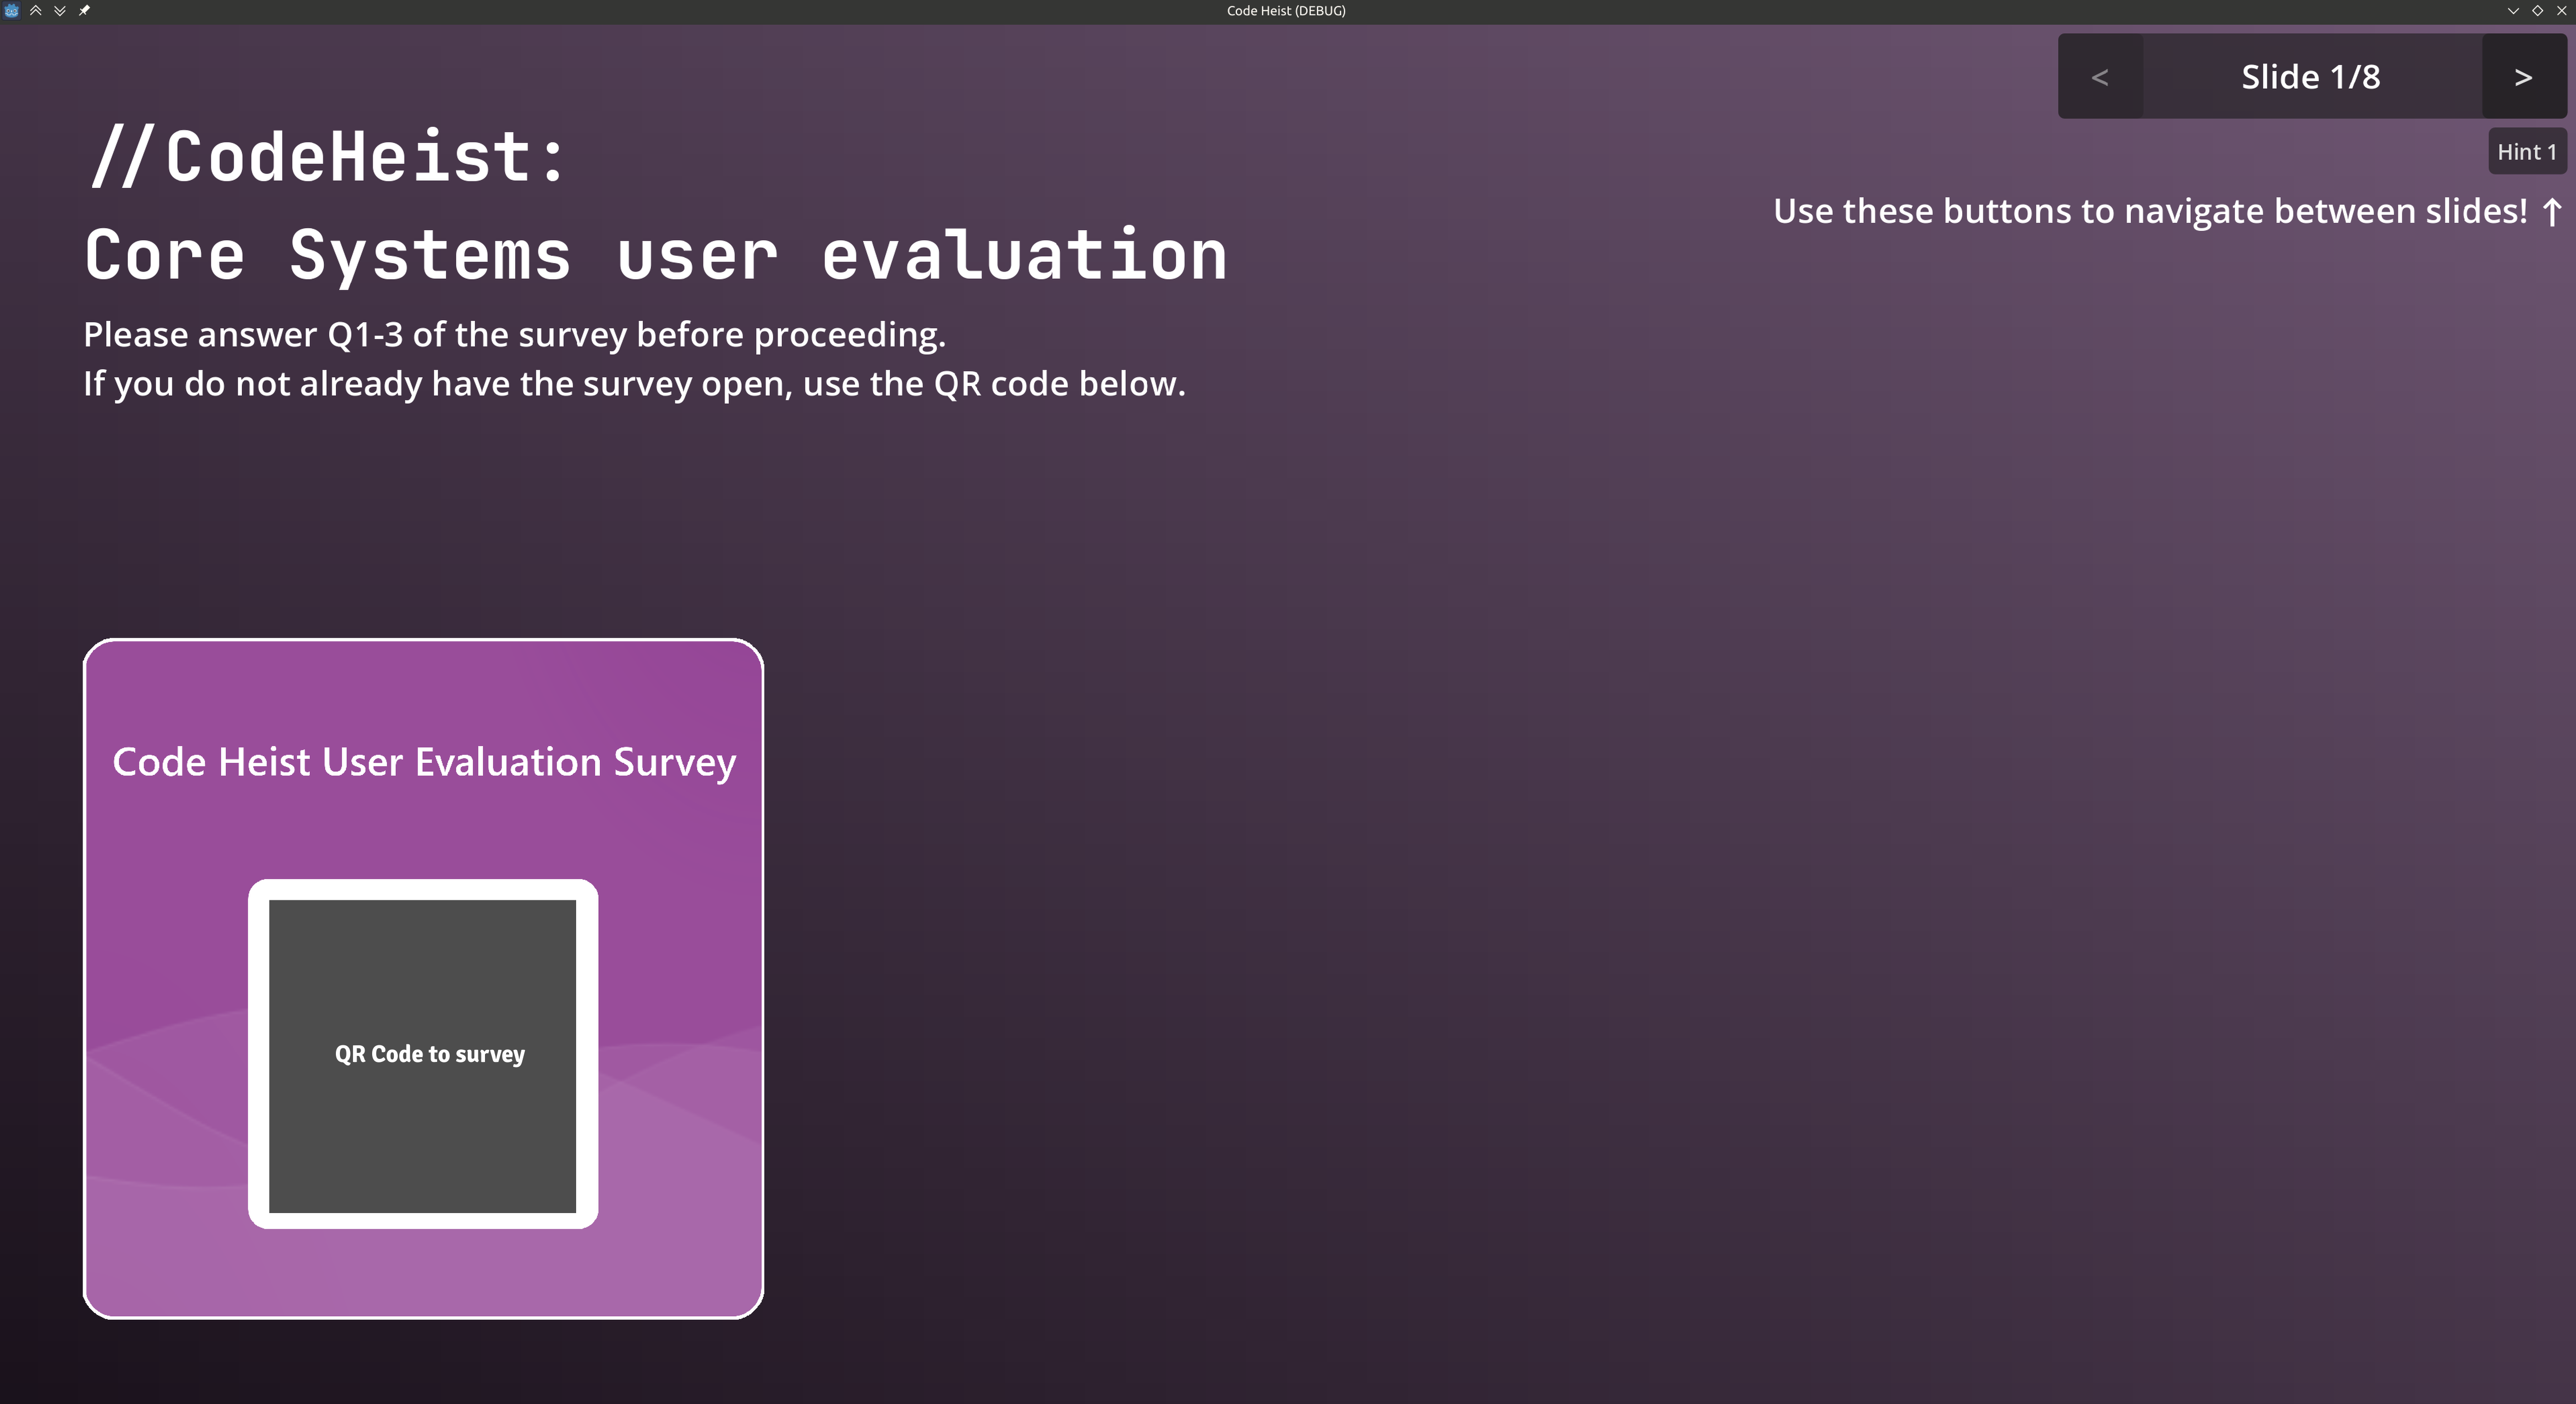
\includegraphics[width=\linewidth]{AE/godotSlide1.png}
    \caption{Screenshot of the Survey Build's slide 1}
\end{figure}

\section{Consent and Background Information}

\subsection{Consent}

Location: \textbf{Microsoft Forms}

This section was made to confirm that a participant consents to taking part in the study, and made it impossible to proceed without doing so.

\begin{fullwidth}
    \begin{quote}
        \textbf{Section 2: Consent}
    
        Title of research project: Code Heist Prototype User Evaluation \\
        Student(s): Drew Rutherford \\
        Module: CM3203 One Semester Individual Project \\
        Module Leader: [Module Leader]
        
        \textbf{Please confirm the following:}
        
        I am above the age of 18. \\
        I have read and understood the information sheet. \\
        I understand that my participation is voluntary and am free to withdraw my consent at any time without giving a reason. \\
        I understand that this study is part of a module and anonymized data may be used included as part of coursework. \\
        I understand that anonymized excerpts and/or verbatim quotes may be used as part of a research publication. \\
        I agree to take part in this research project.

        \textbf{Q1:} I have read and agree to the the above.

        \textit{Options: Confirm}
    \end{quote}
\end{fullwidth}

\subsection{Background Information}

Location: \textbf{Microsoft Forms}

This section was designed to gather the participant's experience with games and programming. This would have been done to measure potential deviation in results between users of different backgrounds.

\begin{fullwidth}
    \begin{quote}
        \textbf{Section 3: Background}
    
        Please answer these questions about your background.

        \textbf{Q2:} How confident are you with programming?

        \textit{Options:}
        \textit{Extremely confident, Somewhat confident, Neutral, Somewhat not confident, Extremely not confident.}

        \textbf{Q3:} How confident are you with video games?

        \textit{Options:}
        \textit{Extremely confident, Somewhat confident, Neutral, Somewhat not confident, Extremely not confident.}
    \end{quote}
\end{fullwidth}

\section{Pre-implemented Controllers}

This section was designed to assess the quality of the movement and controls of CatBot when auto controllers are used. This assesses CR-01, CR-06.1, CR-06.2, CR-07, CR-08 of the \nameref{sec:requirements/core}.

\subsection{Levels}

Location: \textbf{Survey build -- slide 3 - 5}

These levels were designed to be fairly easy, whilst relying on all of the features of CatBot movement:

\textbf{Slide 3:} Horizontal movement, jumping, and semi-solid platforms.

\textbf{Slide 4:} As above, as well as slopes.

\textbf{Slide 5:} As above, as well as strikes, air-strikes and extra camera features.

\begin{figure}[H]
    \centering
    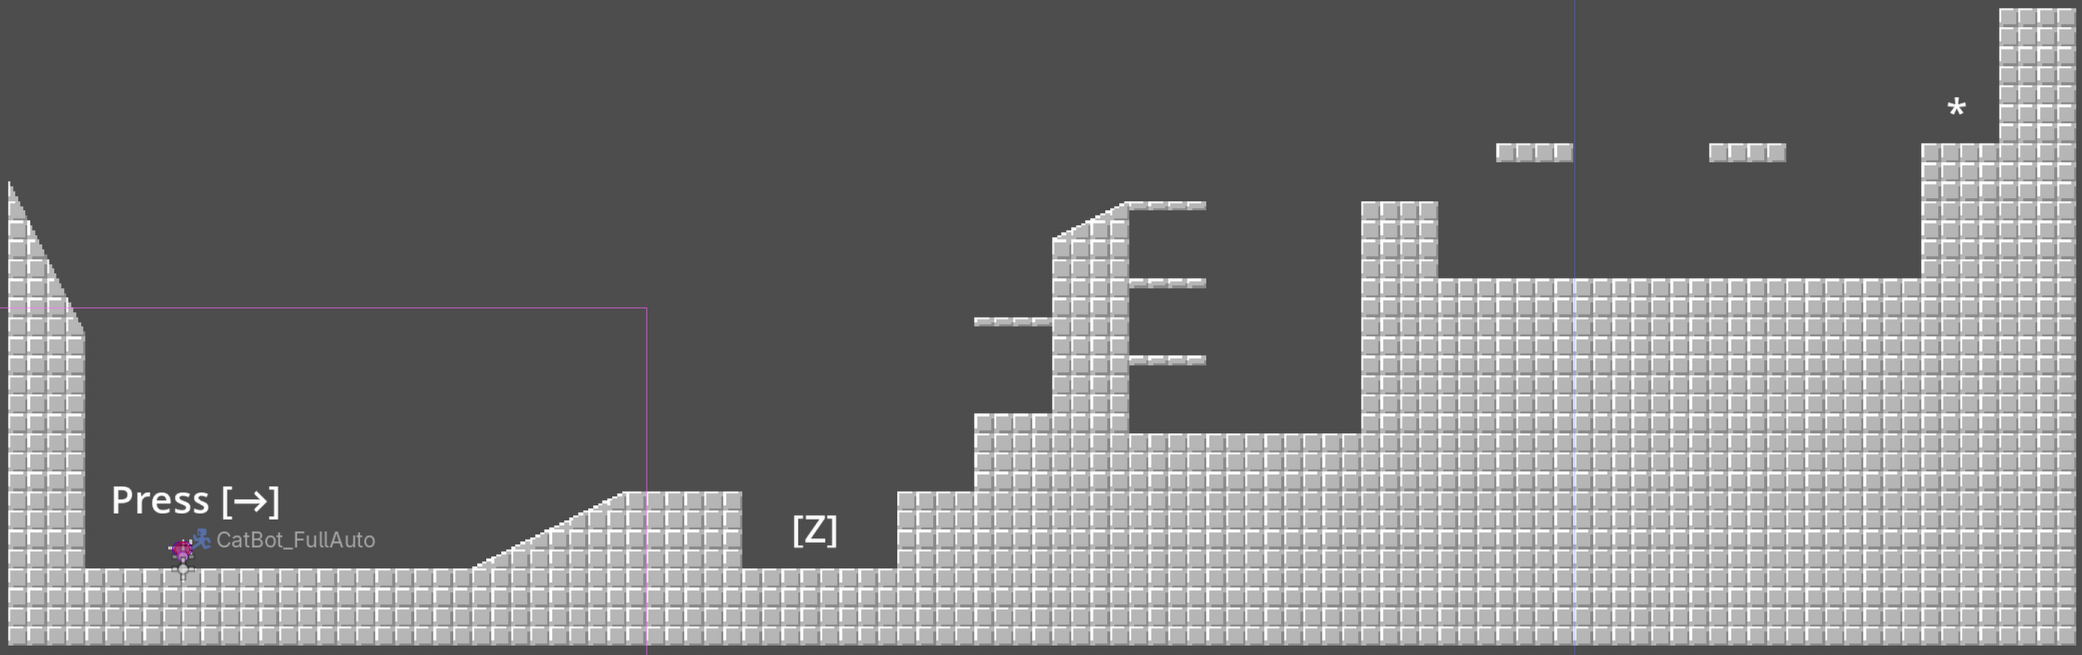
\includegraphics[width=1\linewidth]{AE/godotSlide3.png}
    \caption{Screenshot of the Survey Build's slide 3, in the editor}
\end{figure}

\begin{figure}[H]
    \centering
    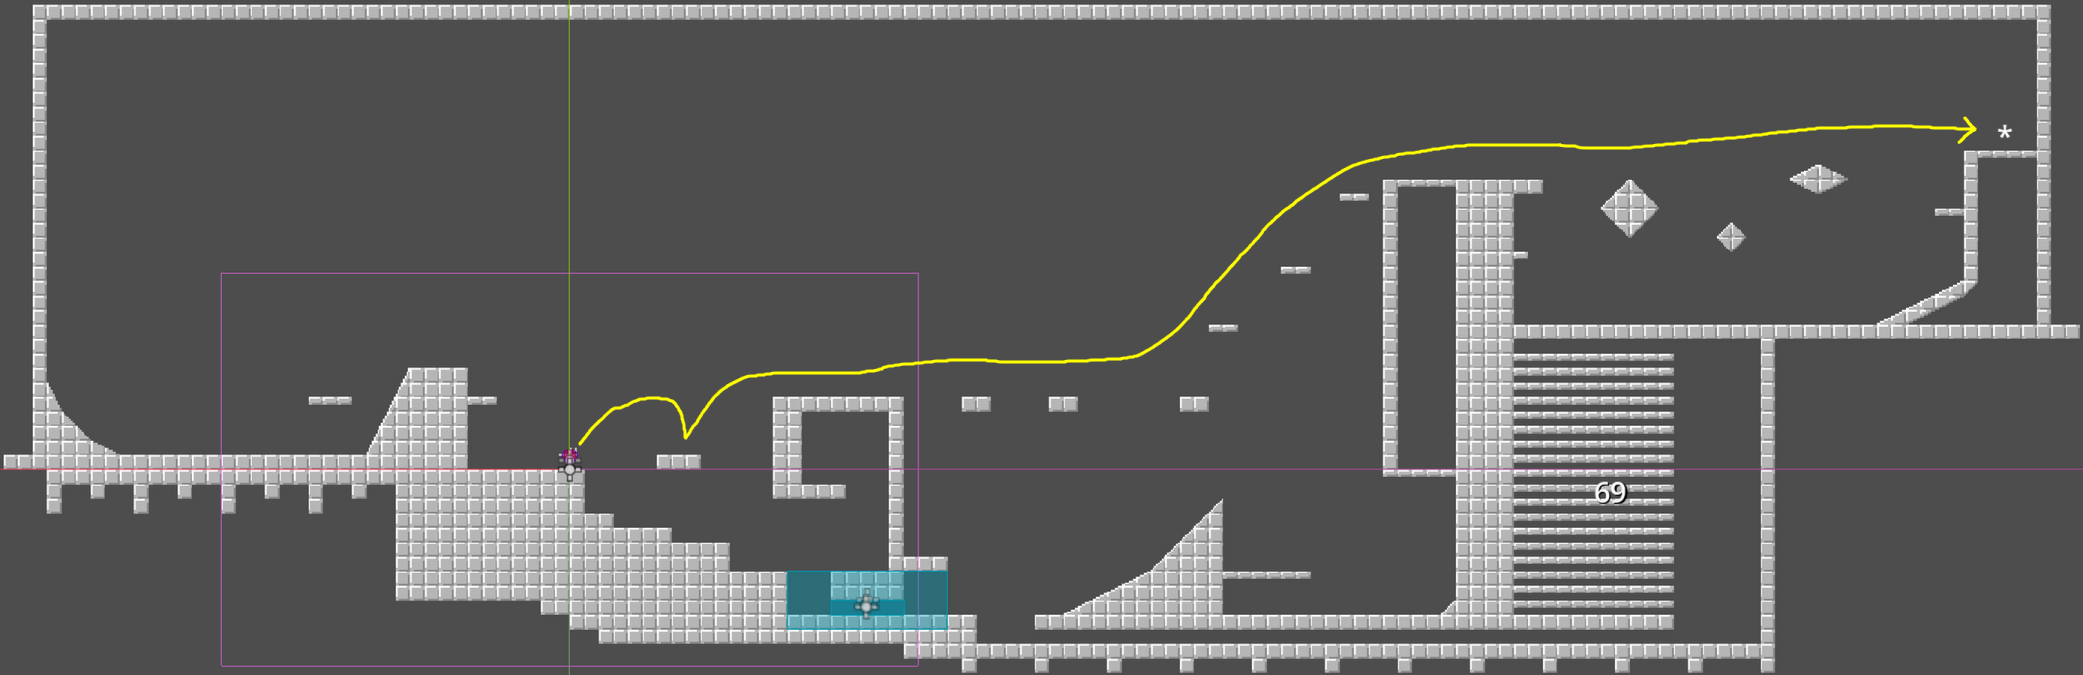
\includegraphics[width=1\linewidth]{AE/godotSlide4.png}
    \caption{Screenshot of the Survey Build's slide 4, in the editor}[Screenshot of the Survey Build's slide 4, in the editor, the critical path shown in yellow]
\end{figure}

\begin{figure}[H]
    \centering
    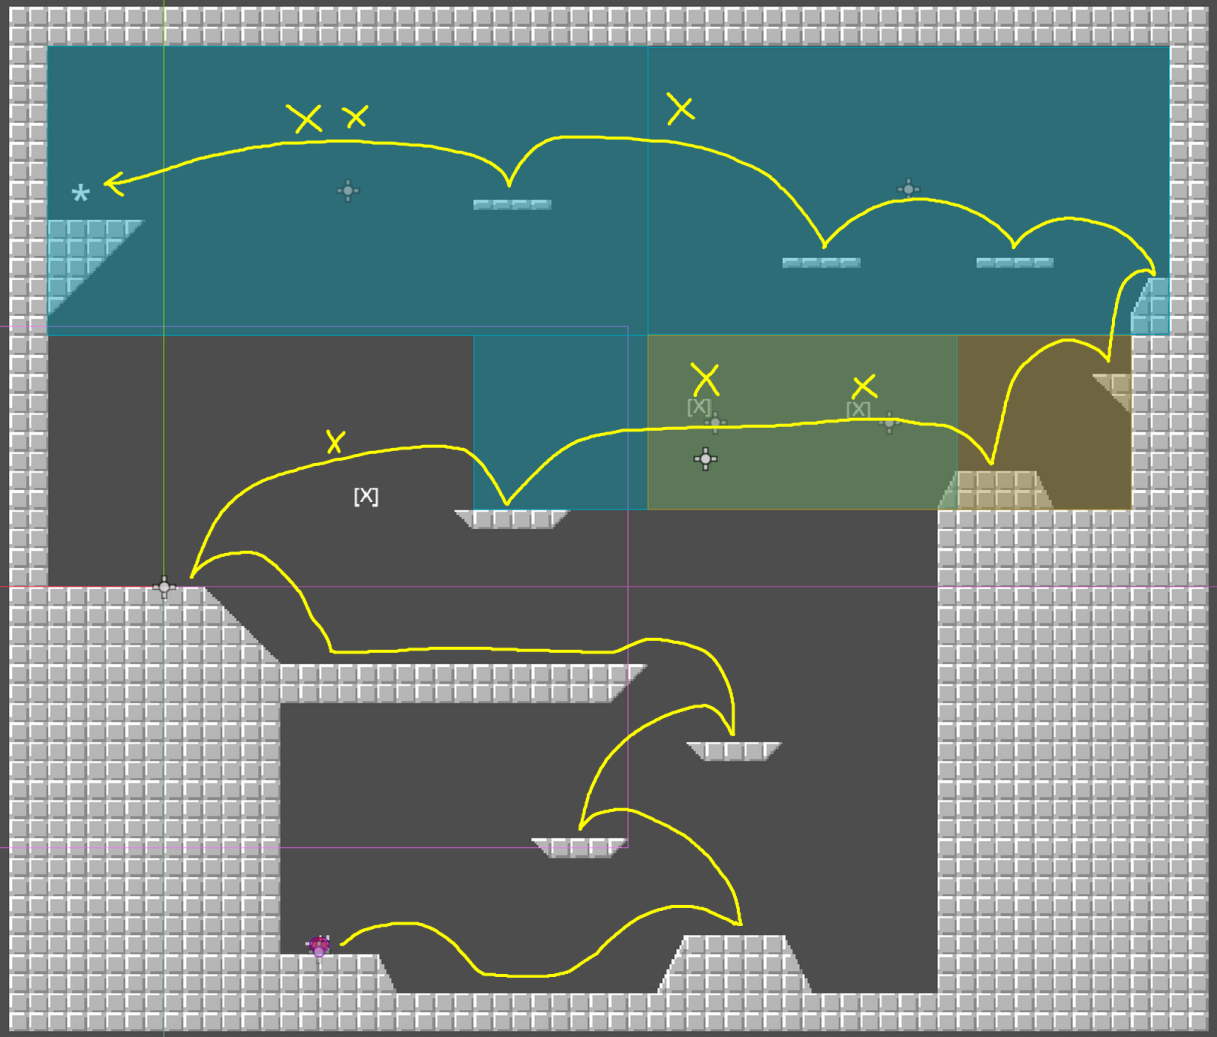
\includegraphics[width=0.65\linewidth]{AE/godotSlide5.png}
    \caption[Screenshot of the Survey Build's slide 5, in the editor]{Screenshot of the Survey Build's slide 5, in the editor, the critical path shown in yellow. Camera modification areas are shown in yellow and blue. Each point where air strikes are marked with an \textquote{x}.}
\end{figure}

\subsection{Questions}

Location: \textbf{Microsoft Forms}

\begin{fullwidth}
    \begin{quote}
        \textbf{Section 4: Automated player controls}
    
        Please play through slides 3 to 5 before answering these questions.

        \textbf{Q4:} To what extent do you agree with the following statements:

        \textit{Options:}
        \textit{Strongly disagree, Disagree, Neutral, Agree, Strongly Disagree.}

        \textbf{Q4-a:} The controls feel intuitive. \\
        \textbf{Q4-b:} The controls feel responsive. \\
        \textbf{Q4-c:} The movement feels fluid. \\
        \textbf{Q4-d:} The physics are fun to play with.

        \textbf{Q5:} If you have any further comment on the programming system, or would like to explain any of your answers please do so here.
    \end{quote}
\end{fullwidth}

\section{CatCoded Controllers}

This section, specifically on the Godot side, was not completed. This section assessed the prototype systems for CatCode and graphical CatCode. This correlates to CR-05, CR-14. CR-15, CR-19, CR-20, CR-21, CR-22, CR-23 of the \nameref{sec:requirements/core}.

\subsection{Levels}

Location: \textbf{Survey build -- slide n - m}

These levels were designed to mirror those from the previous section, except requiring the use of CatCode to re-implement movement.

\textbf{Slide x:} Recreating jumping, requiring \texttt{if}, \texttt{jump()} and some operands.

\textbf{Slide y:} Recreating jumping and striking, requiring more complex logic and \texttt{swipe}.

\textbf{Slide z (unimplemented):} Requires recreating all of CatBot's controllers.

Slide x used the same geometry as slide 3, whilst slide y used the geometry as slide 5, so have not been inlcuded here.

\subsection{Questions}

\begin{fullwidth}
    \begin{quote}
        \textbf{Section 5: CatCode}
    
        Please play through slides x to y before answering the following questions. Feel free to use the hints and solutions or skip slides.

        \textbf{Q6:} To what extent do you agree with the following statements:

        \textit{Options:}
        \textit{Strongly disagree, Disagree, Neutral, Agree, Strongly Disagree.}

        \textbf{Q6-a:} The coding UI is responsive. \\
        \textbf{Q6-b:} The coding UI is intuitive. \\
        \textbf{Q6-c:} I understood what every block does.. \\
        \textbf{Q6-d:} When an error occurred, it is clear why it happened. \\
        \textbf{Q6-e:} When an error occurred, I understood how to fix it. \\
        \textbf{Q6-f:} Creating scripts was enjoyable

        \textbf{Q5:} If you have any further comment on the programming system, or would like to explain any of your answers please do so here.
    \end{quote}
\end{fullwidth}

\section{General Questions}

The final set of questions were more general, attempting to identify any performance issues. It also assessed participant attitudes towards a potential full game.

\subsection{Questions}

Location: \textbf{Microsoft Forms}

\begin{fullwidth}
    \begin{quote}
        \textbf{Section 6: Full Prototype}
    
        These final questions are about your experiences with the entire prototype.

        \textbf{Q8:} Did you experience any performance issues or crashes whilst playing the prototype?

        \textit{Options:}
        \textit{Yes, No, I don't know.}

        \textbf{Q9:} If you answered yes to the previous question, please describe what happened, as well as any hardware details.

        \textbf{Q10:} How interested would you be in playing a completed game incorporating programming elements into its mechanics?

        \textit{Options:}
        \textit{Extremely interested, Somewhat interested, Neutral, Somewhat uninterested, Extremely uninterested}

        \textbf{Q11:} If you have any further comment, please say so here.
    \end{quote}
\end{fullwidth}